\section{Phylogenetics and phylodynamics}

\subsection{Phylogenetic trees}

In evolutionary biology, a \defn{phylogeny}, or \defn{phylogenetic tree}, is a
graphical representation of the the evolutionary relationships among a group of
organisms or species (generally, \defn{taxa})~\autocite{haeckel1866generelle}.
The \defn{tips} of a phylogeny, that is, the nodes without any descendants,
correspond to \defn{extant}, or observed, taxa, while the \defn{internal nodes}
correspond to their common ancestors. The edges or \defn{branches} of the
phylogeny connect ancestors to their descendants. Phylogenies may have a
\defn{root}, which is a node with no descendants distinguished as the most
recent common ancestor of all the extant
taxa~\autocite{harding1971probabilities}. When such a root exists, the tree is
referred to as being \defn{rooted}; otherwise, it is \defn{unrooted}. The
structural arrangement of nodes and edges in the tree is referred to as its
\defn{topology}~\autocite{cavalli1967phylogenetic}. 

The branches of the tree may have associated lengths, representing either
evolutionary distance or calendar time between ancestors and their descendants.
The term ``evolutionary distance'' is used here imprecisely to mean any sort of
quantitative measure of evolution, such as the number of differences between
the DNA sequences of an ancestor its descendant, or the difference in average
body mass or height. A phylogeny with branch lengths in calendar time units is
often referred to as \defn{time-scaled}. In a time-scaled phylogeny, the
internal nodes can be mapped onto a timeline by using the tips of the tree,
which usually map to the present day, as a reference
point~\autocite{nee1992tempo}. The corresponding points on the timeline are
called \defn{branching times}, and the rate of their accumulation is referred
to as the \defn{branching rate}. Rooted trees whose tips are all the same
distance from the root are called \defn{ultrametric}
trees~\autocite{buneman1974note}. These concepts are illustrated in
Figure~\ref{fig:speciestree}.

\begin{figure}[ht]
  \centering
  \label{fig:speciestree}
  \includegraphics{speciestree}
  \caption[Illustration of a rooted, ultrametric, time-scaled phylogeny]
    {Illustration of a rooted, ultrametric, time-scaled phylogeny. The tips of
      the tree, which represent extant taxa, are placed at the present day on
      the time axis. Internal nodes, representing extinct common ancestors to
      the extant taxa, fall in the past. The topology of the tree indicates
      that cats and dogs are the most closely related pair of species, whereas
      fish is most distantly related to any other node in the tree.}
\end{figure}

\subsection{Transmission trees and epidemiology}

In epidemiology, a \defn{transmission tree} is a graphical representation of an
epidemic's progress through a population. Like phylogenies, transmission trees
have tips, nodes, edges, and branch lengths. However, rather than recording an
evolutionary process (speciation), they record an epidemiolgical process
(transmission). The tips of a transmission tree represent infected hosts, while
internal nodes correspond to transmissions from one host to another.
Transmission trees generally have branch lengths in units of calendar time,
with a root corresponding to the index case, and branching times indicating
times of transmission. The internal nodes may be labelled with
the donor of the transmission pair, if this is known. The tips of the tree,
rather than being fixed at the present day, are placed at the time at which the
individual was removed from the epidemic, such as by death, recovery,
isolation, behaviour change, or migration. Consequently, the transmission tree
may not be ultrametric, but may have tips located at varying distances from the
root. Such trees are said to have \defn{heterochronous}
taxa~\autocite{drummond2003measurably}, in contrast to the
\defn{isochronous} taxa found in the phylogenies of macro-organisms.  A
transmission tree is illustrated in Figure~\ref{fig:virustrees}.

\begin{figure}
    \centering
    \includegraphics{virustrees}
    \label{fig:virustrees}
    \caption[Illustration of a transmission tree]{
        A transmission tree representing an epidemic's progress through
        four individuals. The index case, patient $a$, transmitted the
        virus to patients $b$ and $c$; patient $c$ went on to infect
        patient $d$. 
    }
\end{figure}

Since transmission trees are essentially a detailed record of an epidemic's
progress, they contain substantial epidemiological information. As a basic
example, the \gls{ltt} plot~\autocite{nee1992tempo}, which plots the number of
lineages in a phylogeny against time, can be used to quantify the incidence of
new infections over the course of an epidemic~\autocite{holmes1995revealing}.
Many more diverse epidemiological parameters have been investigated using
transmission trees, such as the degree of
clustering~\autocite{hughes2009molecular} and the effect of elevated
transmission risk in acute infection~\autocite{volz2012simple}. However, in all
but the most well-studied of epidemics, this is not possible to obtain through
traditional epidemiological methods. The time and effort to conduct detailed
interviews and contact tracing of a sufficient number of infected individuals
is usually prohibitive. Even when the resources for such methods are available,
patients may not always recall whom they contacted and when, especially in the
case of airborne transmission. Consequently, the transmission tree must be
estimated using other methods. Most commonly, this is done by exploiting the
relationship between transmission trees and viral phylogenies.

\subsection{Estimating transmission trees from viral phylogenies}

In general, \defn{viral phylogenies} are simply phylogenetic trees relating
virus strains. \comment{Is ``strain'' the best word here?} In phylodynamics, we
often consider \defn{inter-host} phylogenies, which relate one viral genotype
from each host in a population. The tips of the tree are labelled with both the
virus and its host. The crux of
\defn{phylodynamics}~\autocite{grenfell2004unifying} is the fact that the
processes generating these two types of tree - epidemiological processes, for
transmission trees, and evolutionary processes, for viral phylogenies - occur
on similar time scales for RNA viruses~\autocite{drummond2003measurably}. As a
result, there is a close relationship between the two trees. In particular, the
transmission process is quite similar to \defn{allopatric
speciation}~\autocite{coyne2004speciation}, where genetic divergence follows
the geographic isolation of a sub-population of organisms. Thus, transmission,
which is represented as branching in the transmission tree, causes branching in
the viral phylogeny as well. Similarly, the removal of an individual causes the
extinction of their viral lineage. Due to these relationships, the topology of
the viral phylogeny is often used as a proxy for the topology of the
transmission tree. However, there are several complications and caveats which
must be kept in mind when estimating the transmission tree in this manner.

First are the issues of rooting and time-scaling. Modern likelihood-based
methods of phylogenetic reconstruction produce unrooted trees whose branch
lengths measure genetic distance in units of expected substitutions per site,
whereas transmission trees are rooted with branches measuring calendar time.
We generally assume that sampling a virus from the individual also corresponds
to their removal from the transmission tree\comment{needs a reference}, so the
positions of the tips in time are fixed. Therefore, to transform a viral
phylogeny into an estimated transmission tree, we must find a root and an
assignment of branch lengths such that the tips are placed at their proscribed
times. Of course, there are an infinite number of possible combinations of root
and branch lengths which result in the correct placement of the tips, so we
would also like to find values which are the most ``reasonable'' given our
data. By reasonable, we mean that the variation in \defn{evolutionary rate}, 
which is the ratio of a branch's length in genetic distance to its length in
calendar time, is low across the tree. While there is some variation among
hosts, due to immunological and other factors, we generally expect to observe
globally similar evolutionary rates. Methods for time-scaling a phylogeny
include root-to-tip regression~\autocite{drummond2003inference}, which we apply
in this work, and least-square dating~\autocite{to2015fast}. Both of these
methods can be used to root the tree, by simply trying all possible root
positions and choosing the one which minimizes a loss function
($1-R^2$ or root-mean-square error for root-to-tip regression, sum of squared
errors for least-square dating). Alternatively, the tree may be rooted with an
outgroup before time-scaling.

A second, perhaps more insidious problem is the fact that the correspondence
between the topologies of the viral phylogeny and transmission tree is not
necessarily exact. Due to intra-host diversity, the viral strain which is
transmitted may have split from another lineage within the donor long before
the transmission event occurred. Hence, the branching point in the viral
phylogeny may be much earlier than that in the transmission tree. Another
possibility is that one host transmitted to two or more recipients, but the
lineages they each received originated within the donor host in a different
order than that in which the transmissions occurred. In this case, the topology
of the transmission tree and the viral phylogeny will be mismatched. Although
phylodynamics is quite new, these phenomena have been studied in evolutionary
biology for some time. Viral phylogenies are a specific version of a more
general class of trees called \defn{gene trees}, which represent the
evolutionary history of a section of genetic material. Transmission trees, on
the other hand, are highly analogous to \defn{species trees}, whose tips are
species and internal nodes are common ancestors. This analogy derives from the
functional similarity between transmission and allopatric speciation. Hence,
the potential discordance between transmission trees and viral phylogenies is
the similar to that between gene and species trees, which is called
\defn{incomplete lineage sorting}. In practice, this discordance has not proven
an insurmountable problem: for example, \textcite{leitner1996accurate} were
able to accurately recover a known transmission tree using a viral phylogeny.

A final caveat is that the viral phylogeny itself is not known with certainty,
so it must also be estimated from genetic data. Phylogenetic inference is a
complex topic which we will not discuss in detail here (see e.g.
\autocite{nei2000molecular} for a full review). Most modern analyses use
model-based methods, which simultaneously estimate the phylogeny with branch
lengths and the parameters of a model of evolution. Although they usually work
well in practice \comment{needs a reference}, the estimated topology can vary
based on the model used and, in the case of Bayesian analysis, the priors.  In
addition, intra-host viral populations are genetically heterogeneous, so
choosing a single representative genotype per host is necessarily imprecise.
One can use either the genotype of a specific virion sampled from the host, or
a synthetic genotype, such as a consensus or reconstructed ancestral sequence.

What we have just discussed is a two-step procedure for estimating the
transmission tree. First, a viral phylogeny is constructed from genetic
sequence data, and then it is rooted and time-scaled into a transmission tree.
This approach is straightforward, frequently used, and has the advantage of
leveraging tried-and-true tools for phylogenetic inference. However, it also
has drawbacks, perhaps the most obvious being the multiplication of errors
produced by the separate steps. One commonly used alternative method is to
directly estimate a time-scaled phylogeny by simultaneously inferring the tree
topology, its root and branch lengths, and the parameters of a \defn{molecular
clock} model. A molecular clock is a hypothesis about the evolutionary rates
along the branches of the tree, such as that they are all equal (a \defn{strict
clock}) or that they are \gls{iid} from a common distribution (a \defn{relaxed
clock}). This inference is usually done in a Bayesian framework using
\gls{MCMC}, so that prior information (including the tip dates) \comment{are
tip dates part of the prior?} can be included in the analysis, and the
so-called nuisance parameters of the molecular clock model can be marginalized
out. Software packages for performing these analyses include
BEAST~\autocite{bouckaert2014beast} and MrBayes~\autocite{ronquist2012mrbayes}.

Several other authors have developed methods tailor-made for inferring
transmission trees. \textcite{didelot2014bayesian} develop a Bayesian version
of the two-step approach which allows transmissions to occur anywhere along the
branches of a transmission tree, rather than being constrained to the branching
points in the viral phylogeny. The method requires sampling of every infected
individual, although the authors indicate that it could be extended to relax
this assumption. \textcite{cottam2008integrating} describe a likelihood-based
method which enumerates all transmission trees consistent with an established
phylogeny, assigning each a likelihood based on other epidemiological data. 
This approach is novel in its integration of data from multiple sources,
however because it enumerates a large portion of the tree space, it is unlikely
to scale to larger epidemics. A different approach is undertaken by
\textcite{jombart2011reconstructing}, who describe a method to build
transmission trees directly from sequence data, contingent on the common
ancestors also being sampled. This makes the method attractive for
slow-evolving pathogens, but less practical for viral outbreaks where samples
from common ancestors are unlikely to be available.

%\subsection{Species trees and transmission trees}
%\label{subsubsec:speciestree}
%
%A \defn{species tree} is a particular type of phylogeny in which the taxa are
%species, and the branching times correspond to historical speciation events. By
%speciation events, we mean times when two formerly interbreeding groups of
%organisms ceased to reproduce with each other. In general, we do not have
%access to the true tree relating a particular group of extant species, as this
%would usually imply certain knowledge of speciation events in the distant past.
%Therefore, all species trees considered by researchers are estimates, based on
%the genetic or phenotypic similarity of the extant taxa, the fossil record, or
%both. We discuss some of the challenges associated with this estimation in
%subsection \ref{subsubsec:treeconv} below. However, for the moment, we ignore
%these complications and consider what can be said about the true species tree.
%
%Speciation often occurs by an \defn{allopatric} process, where a sub-population
%of organisms is isolated from the original population by a geographic
%barrier~\autocite{coyne2004speciation}. Over time, differing selection
%pressures on either side of the barrier, coupled with genetic drift, cause the
%two populations to diverge genetically. This eventually results in two distinct
%species, which will appear as two subtrees or \defn{clades} in their species
%tree if descendants of both survive to the present. Of course, this is not
%necessarily the case, as selection may cause one or both of the new
%sub-populations or their descendants to become extinct. On the other hand,
%selection may favour one of the sub-populations, allowing it to expand into new
%regions or niches and possibly paving the way for subsequent speciation events.
%Speciation is not necessarily allopatric: \defn{sympatric} speciation refers to
%the emergence of a new species without any geographic
%barrier~\autocite{coyne2004speciation}. Indeed, there is a whole continuum of
%possible speciation processes~\autocite{fitzpatrick2008if}, ranging from
%completely allopatric to completely sympatric. However, at least for eukaryotic
%organisms, allopatric speciation is thought to be by far the most common
%type~\autocite{coyne2004speciation}. 
%
%At first glance, transmission trees and species trees seem to have nothing to
%do with each other. One represents the evolutionary history of a group of
%organisms, the other traces the spread of a disease through a host population.
%However, when considering epidemics of RNA viruses, transmission trees and
%species trees are highly related. The viral population within a single host has
%often been referred to as a \defn{quasispecies}~\autocite{domingo2012viral},
%and due to the fast evolutionary rate of these viruses, two hosts' viral
%populations are invariably genetically distinct. The transmission process is
%functionally identical to allopatric speciation, involving geographic isolation
%of a sub-population in a new host and subsequent genetic divergence. However,
%for the most part, it is not selection but rather host epidemiology which
%causes certain lineages to proliferate while driving others to extinction. A
%host who recovers, dies, or is isolated equates to an extinction in the
%transmission tree. On the other hand, dense populations in frequent contact
%often experience rapid epidemic growth, which causes similarly rapid
%accumulation of branching points in the tree. 
%
%The fact that these evolutionary (ie. speciation) and epidemiological processes
%occur on the same time scale for RNA viruses~\autocite{drummond2003measurably}
%is the basis for the field of
%\defn{phylodynamics}~\autocite{grenfell2004unifying}. The similarity between
%transmission and speciation means that it is possible to apply many of the
%tools and techniques developed for species trees to viral transmission trees,
%and interpret the results in the context of transmission rates and host
%epidemiology. 
%
%%As a basic example, the lineages-through-time
%%plot~\autocite{nee1992tempo}, which plots the historical speciation rate
%%against time, can be used to quantify the incidence of new infections over the
%%course of an epidemic~\autocite{holmes1995revealing}. 
%In
%subsection~\ref{subsubsec:treeshape} below, we review some of these methods in
%more detail, as well as several which have been developed specifically for
%viral phylodynamics, and discuss what these methods can tell us about host
%epidemiology.
%
%Finally, we must note two important points. First, we have not yet considered
%the selection pressures operating within a single host, such as the immune
%response. Second, we reiterate that both transmission trees and species trees
%are theoretical objects which are almost never known with certainty for real
%data. Indeed, the estimation of transmission trees is often problematic, and it
%is in such estimation that within-host forces play a role. Both of these issues
%are discussed further below in subsection~\ref{subsubsec:treeconv}, though we
%continue to ignore them in the next subsection.
%
%\subsection{Gene trees and viral phylogenies}
%\label{subsubsec:genetree}
%
%A \defn{gene tree} is another type of phylogeny which traces the evolutionary
%history of one or more sections of genetic material. Gene trees can be built
%from small parts of genes up to whole genomes, but for ease of exposition we
%will use only the word ``gene''. The tips of a gene tree represent the
%different \defn{alleles}, or versions, of the gene found in the studied taxa.
%The branching points in a gene tree represent genetic divergence events - that
%is, the times when two distinct alleles first came into existence through
%mutation.
%
%Gene trees are usually estimated using the nucleotide or amino acid sequences
%of the genes in question. Although there are methods for estimating gene trees
%using other types of molecular data, such as gene orders, we will focus on
%sequence-based methods here. As with species trees, it is not possible to know
%gene trees with certainty, only to estimate them. However, the problem of
%estimating gene trees directly from data is somewhat better defined than that
%of estimating species trees, because of the quantitative nature of the
%molecular data used to label the tips. In general, methods to estimate gene
%trees fall into three major categories: distance-based, maximum parsimony, and
%model-based. The first two categories are generally
%no longer used for phylogenetic inference, since model-based methods have been
%demonstrated to be almost universally more accurate. Therefore, we will review
%in detail only the last category.
%
%Model-based methods include both maximum likelihood and Bayesian approaches. To
%use them, one must first define a parametric model of sequence evolution, here
%denoted $M$. For all possible trees $T$ (with branch lengths) and choices of
%model parameters $\theta$, the model must define a probability density function
%on observed sequence data $D$, denoted $f(D \mid T,\,\theta)$. This is also
%sometimes written $\Pr(D \mid T,\,\theta)$, even though it is a probability
%\emph{density}, not a probability. Maximum likelihood aims to find a particular
%tree and values for the model parameters which optimize the \defn{likelihood
%function} $\L$ for the observed data,
%\[
%  \L(\theta,\, T \mid D) = f(D \mid T,\, \theta).
%\]
%Bayesian methods, rather than trying to find point estimates for $\theta$ and
%$T$, aim to approximate the entire \defn{posterior distribution} for the
%observed data,
%\[
%  f(T,\,\theta \mid D) = \frac{f(D \mid T,\,\theta)f(T,\,\theta)}{f(D)}.
%\]
%Here, $f(T, \theta)$ denotes the prior distribution on $T$ and $\theta$, and
%$f(D)$ is the marginal density of the data (that is, the integral of the
%numerator over all values of $T$ and $\theta$).
%
%\subsection{Estimating transmission trees}
%\label{subsubsec:treeconv}
%
%Most applications of viral phylodynamics, including this project, aim to answer
%epidemiological questions~\autocite{pybus2009evolutionary, volz2013viral}. 
%For example, phylodynamic methods have been used to investigate the degree of
%clustering~\autocite{hughes2009molecular} and the effect of elevated
%transmission risk in acute infection~\autocite{volz2012simple} 
%(a more thorough
%review is given below in subsection~\ref{subsubsec:appphylo}). For these
%applications, we are ultimately interested in the transmission tree, which is a
%representation of an epidemiological process (transmission), as opposed to the
%viral phylogeny, which represents a biological process (viral evolution). As
%discussed above in subsection~\ref{subsubsec:speciestree}, transmission trees
%and are in practice unknown, and must be estimated from available data. Here,
%we review some of the ways to perform such estimation.
%
%In principle, transmission trees can be reconstructed by on-the-ground
%epidemiological methods, that is, by asking each person who they contacted.
%This is particularly relevant for sexually transmitted diseases such as HIV,
%where individuals are more likely to recall who they contacted and
%when~\autocite{klovdahl1985social}. This kind of data is challenging to collect
%in detail. Most commonly, when applying phylodynamics in practice, the
%transmission tree is estimated from the viral
%phylogeny~\autocite{volz2013viral}. As discussed above in
%subsection~\ref{subsubsec:genetree}, the viral phylogeny is itself also estimated;
%however, for the moment we ignore this complication and describe methods for
%estimating the transmission tree if the viral phylogeny were known.
%
%When we consider the fact that the viral phylogeny is not known with certainty,
%the methods just described follow a two-step procedure. The first step is to
%estimate the viral phylogeny, and the second step is to use it to estimate the
%transmission tree.
%
%\autocite{didelot2014bayesian} develop a Bayesian version of the two-step
%approach. They first estimate a time-scaled phylogeny from viral samples, then
%estimate the transmissions which took place along the phylogeny. Due to
%within-host evolution, the transmissions are allowed to occur anywhere along
%the branches, rather than being constrained to happen at branching points.
%However, the authors admit that their method requires sampling of every
%infected individual, although they indicate that it could be extended to relax
%this assumption.
%
%A different approach is undertaken by Jombart
%\etal~\autocite{jombart2011reconstructing}, who build transmission trees
%directly from sequence data without the intermediate step of constructing a
%phylogeny. Their method finds the most likely geneology among the sampled
%sequences, assuming that the that the common ancestors to sampled isolates are
%themselves sampled. Although this may be a realistic assumption in the early
%stages of an epidemic of a slower evolving pathogen, it is unlikely for
%ancestors to be present among sequences sampled from an ongoing HIV epidemic
%\comment{Needs a reference}.
%
%Several alternative approaches have been developed which aim to
%incorporate available epidemiological data as well. Cottam
%\etal~\autocite{cottam2008integrating} first built a viral phylogeny, then
%enumerated all transmission trees consistent with this phylogeny by labelling
%the internal nodes of the phylogeny in every possible way. Each of the putative
%transmission trees was assigned a likelihood based on infection time and
%geographic separation. 
%
%


\newpage

\subsection{Tree shapes}
\label{subsubsec:treeshape}

The aim of viral phylodynamics is to glean some kind of knowledge, about the
epidemic, the virus, or its hosts and their behaviour, by studying a phylogeny,
most often a transmission tree~\autocite{pybus2009evolutionary, volz2013viral}.
Phylogenies are complex objects, and it is not immediately obvious how to
extract useful information from them with respect to fitting a parameter.
Standard statistical methods built for numeric data cannot be applied directly
- for example, one cannot perform a regression of a parameter of interest
against a phylogeny. Therefore, before we discuss exactly what phylodynamics
can tell us about epidemics, and how it has been applied in the past, we will
review some of the methods for quantifying the shapes of phylogenies and their
similarity to each other.

Many tree summary statistics have been developed to assign numerical values to
phylogenies based on their properties. One of the most widely used is Sackin's
index~\cite{shao1990tree}, which measures the imbalance or asymmetry in a
rooted tree. For the $i$th tip of the tree, we define $N_i$ to be the number of
branches between that tip and the root. The unnormalized Sackin's index is
defined as the sum of all $N_i$. It is called unnormalized because it does not
account for the number of tips in the tree. Among two trees having the same
number of tips, the least-balanced tree will have the highest Sackin's index.
However, among two equally balanced trees, the larger tree will have a higher
Sackin's index. This makes it challenging to compare balances among trees of
different sizes. To correct this, \textcite{kirkpatrick1993searching} derive
the expected value of Sackin' index under the Yule
model~\autocite{yule1925mathematical}. Dividing by this expected value
normalizes Sackin's index, so that it can be used to compare trees of different
sizes.

An alternative to summary statistics are \defn{distance measures} on trees.
Rather than assigning a numerical value to each tree individually, a distance
measure associates each pair of trees with a number, indicating how different
the trees are from each other. Distance measures allow us to identify groups of
related phylogenies, for example, local epidemics which are undergoing a
similar pattern of expansion. One such distance measure is the
\gls{nltt}~\autocite{janzen2015approximate}, which compares the
\gls{ltt}~\autocite{nee1992tempo} plots of two trees. Specifically, the two
\gls{ltt} plots are normalized so that they begin at $(0, 0)$ and end at $(1,
1)$, and the difference between the two plots is integrated between 0 and 1.
In the context of infectious diseases, the \gls{nltt} is related to the
prevalence~\autocite{holmes1995revealing}, so large values may indicate that
the trees being compared are the products of different epidemic
trajectories~\autocite{janzen2015approximate}.

Another tree distance measure is the \defn{phylogenetic kernel}, or ``tree
kernel'' developed by \textcite{poon2013mapping}. Strictly speaking, the tree
kernel is a \defn{similarity measure}, rather than a distance measure, as it is
maximized when the two trees being compared are the same. The basis of the tree
kernel is the kernel trick originally developed for
\glspl{SVM}~\autocite{burges1998tutorial}. The idea of the kernel trick is to
compare objects by mapping them into a feature space of very high, possibly
even infinite, dimension. The similarity between objects is taken to be their
dot product in the feature space. It is called a ``trick'' because this dot
product is computed using a \defn{kernel function} without explicitly mapping
the objects to the feature space, which would be computationally prohibitive. In
the case of the tree kernel, the feature space is the space of all possible
\defn{subset trees}, which are subtrees that do not necessarily extend all the
way to the tips. The subset-tree kernel was originally developed for comparing
parse trees in natural language processing~\autocite{collins2002new} and did
not incorporate branch length information. The version developed by
\textcite{poon2013mapping} includes a radial basis function to compare the
differences in branch lengths, thus incorporating both the trees' topologies
and their branch lengths in a single similarity score. The tree kernel was
later shown to be highly effective in differentiating trees simulated under a
compartmental model with two risk groups of varying contact
rates~\autocite{poon2015phylodynamic}. In that paper,
\citeauthor{poon2015phylodynamic} used the tree kernel as the distance function
in \gls{ABC} (see Section~\ref{sec:abc}), an approach dubbed kernel-\gls{ABC},
to fit epidemiological models to observed trees.

\subsection{Applications of phylodynamics}
\label{subsubsec:appphylo}


\section{Contact networks}
\label{subsec:contactnet}

\subsection{Overview}

Epidemics spread through populations of hosts through \defn{contacts} between
those hosts. The definition of contact depends on the mode of transmission of
the pathogen in question. For an airborne pathogen like influenza, a contact
may be simple physical proximity, while for a sexually transmitted pathogen
like HIV, contacts would be sexual partnerships. A \defn{contact network} is a
graphical representation of a host population and the contacts among its
members. The \defn{nodes} in the network represent hosts, and \defn{edges}
represent contacts between them. 

Edges in a contact networks may be \defn{directed}, representing one-way
transmission risk, or \defn{undirected}, representing symmetric transmission
risk. For example, a network for an airborne epidemic would use undirected
edges, because the same physical proximity is required for a host to infect or
to become infected. However, a blood-borne infection spread through
transfusions would use undirected edges, since the donor has no chance of
transmitting to the recipient. Directed edges are also useful when the
transmission risk is not equal between the hosts, such as with HIV
transmission, where acting as the receptive partner carries a higher risk of
infection than acting as the insertive partner. In this case, a contact could
be represented by two directed edges, one in each direction between the two
hosts, with the edges annotated by what kind of risk they imply. In fact, it is
possible to represent an undirected edge by two symmetric directed edges. For
this reason, we consider only contact networks with directed edges in the
sequel. A directed contact network is shown in Figure \ref{fig:contactnet}
(left).

The path an epidemic takes through a contact network determines the topology of
the transmission tree relating the infected hosts. The initially infected node
who introduces the epidemic becomes the root of the tree. Each time a
transmission occurs, the lineage corresponding to the donor host in the tree
splits into two, representing the recipient lineage and the continuation of the
donor lineage. This correspondence is illustrated in figure
\ref{fig:contactnet}. It's important to note that, although the order and
timing of transmissions determines the tree topology uniquely, the converse
does not hold. That is, there are generally several orders of infection which
could lead to the same topology, since the labels on the internal nodes of the
tree are not available to the researcher.

\begin{figure}[ht]
  \centering
  \label{fig:contactnet}
  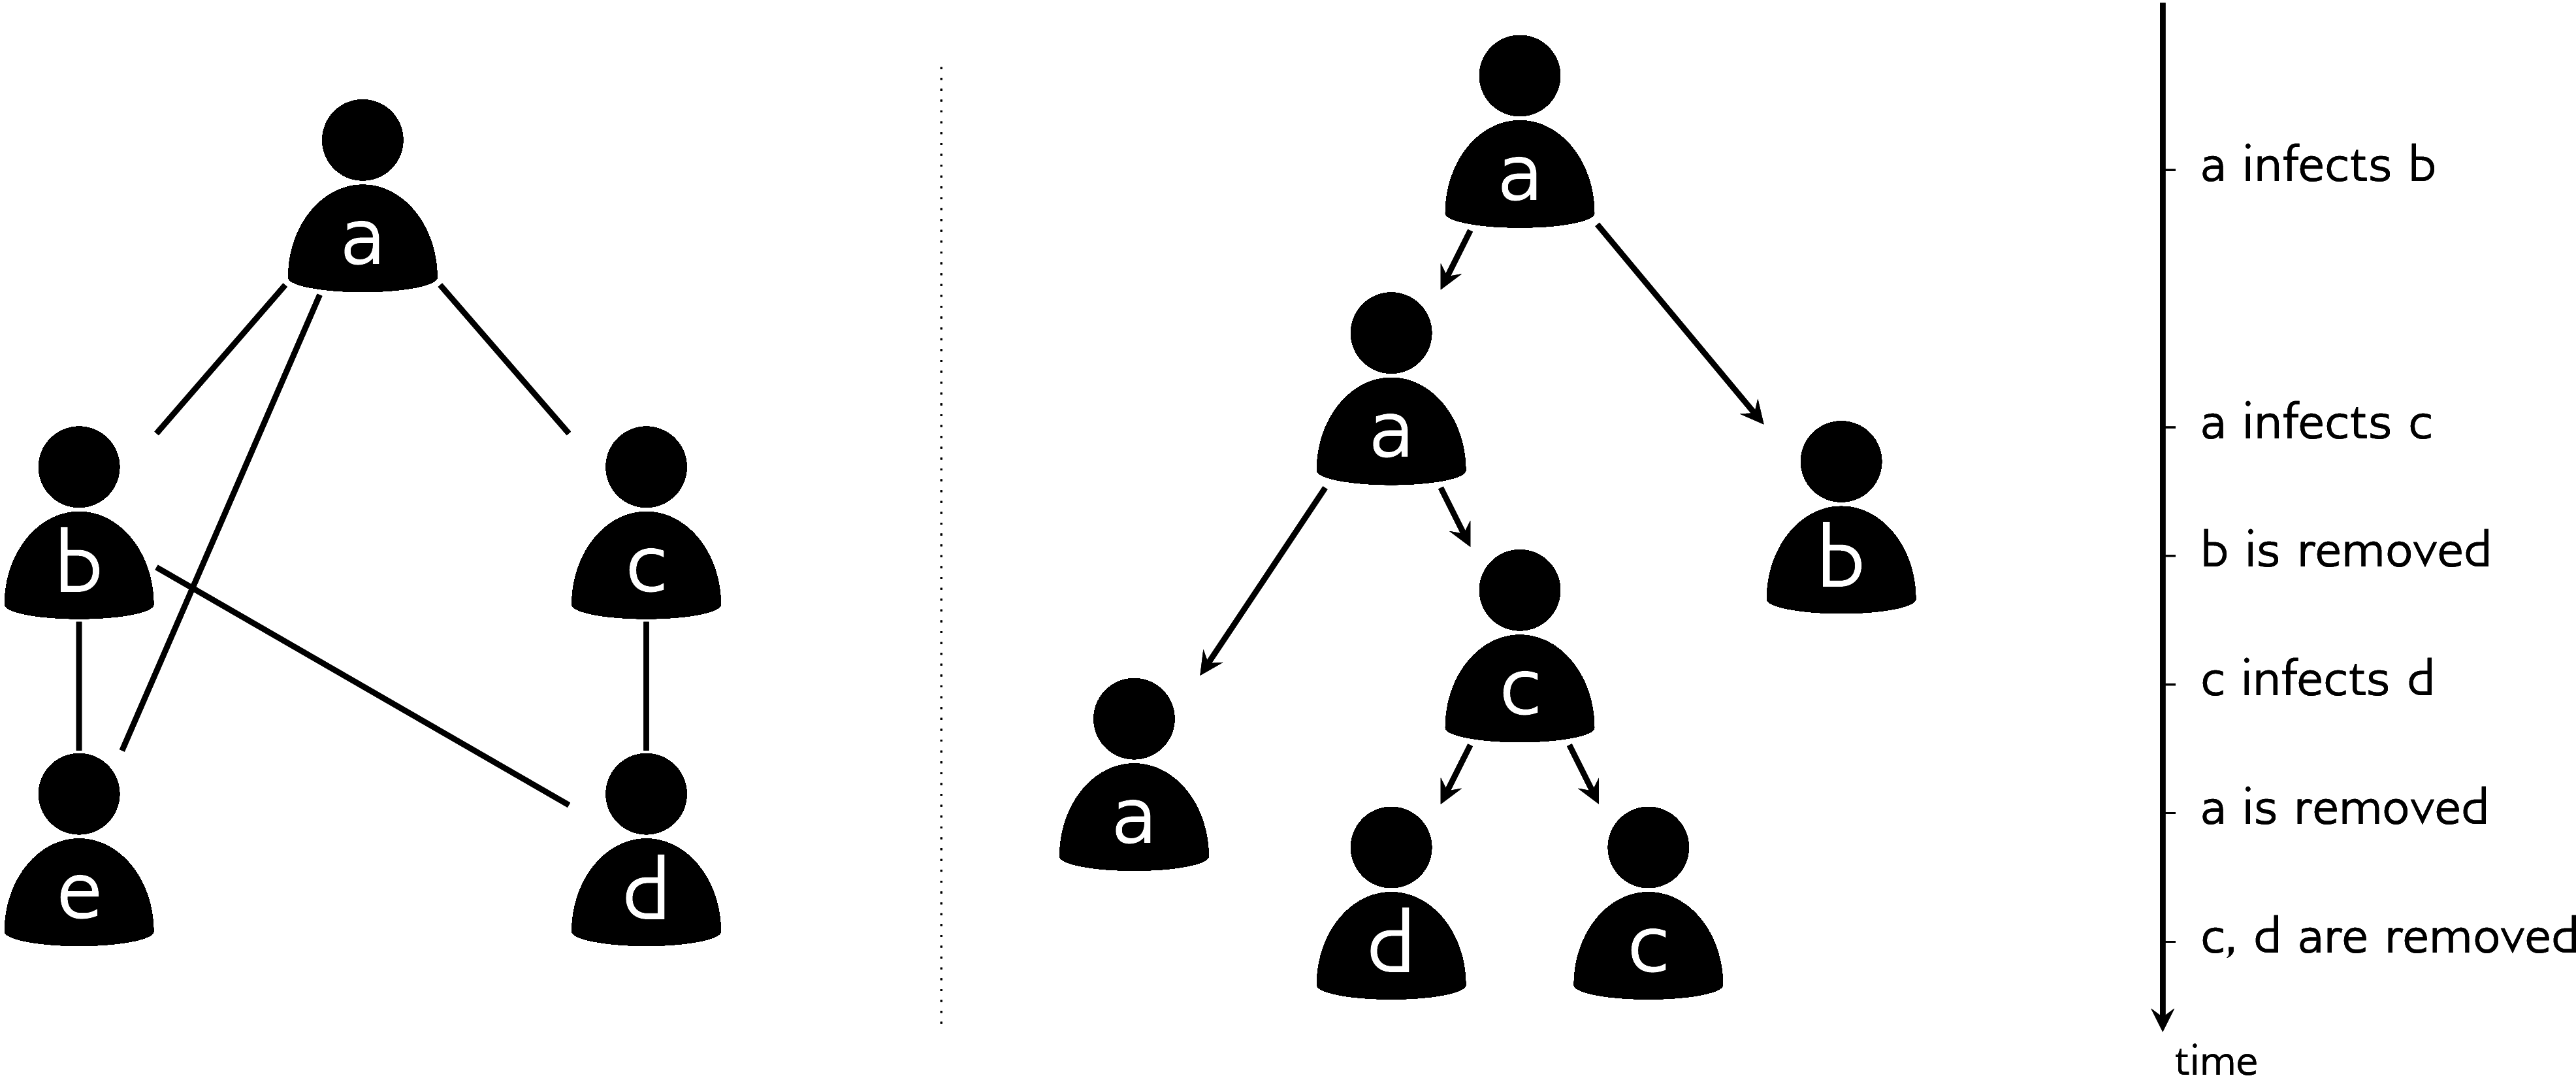
\includegraphics{contactnet}
  \caption[Illustration of a epidemic spread over a contact network]
  {Illustration of epidemic spread over a contact network. On the left, a
   contact network with five hosts, labelled A through E. Directed edges
   indicate six symmetric contacts among the hosts. Coloured, bolded edges
   represent transmissions. The epidemic began with node A, who transmitted to
   nodes B and C. Node C further transmitted to node D, and node E was not
   infected. On the right, the transmission tree topology corresponding to this
   scenario. Note that individual B was sampled before the other infected
   individuals, resulting in a tree with heterochronous tips.}
\end{figure}

\subsection{Models for contact networks}
\label{subsubsec:generative}

Throughout this section, the variable $n$ will be used to refer to the number
of nodes in the network. 

An \defn{Erd\H{o}s-R\'enyi} (ER) network~\autocite{erdos1960evolution}, also
known as a Bernoulli network, was the first network model described. It has a
single parameter, $p$, which is the probability that any particular edge is
present in the network. To construct an ER network, one simply chooses
$p \times \binom{n}{2}$ distinct pairs of nodes and draws an edge between each
pair. The average degree of a node in an ER network is equal to $p \times n$.

A \defn{Barab\'asi-Albert} (BA) network~\autocite{barabasi1999emergence},
incorporates the phenomenon of \defn{preferential attachment} seen in real life
networks. This means that new connections are more likely to involve nodes
which already have a high number of connections - popular nodes tend to become
more popular. In the formulation we consider here, BA networks have two
parameters, $m$ and $\alpha$, which are used to construct the network via the
following algorithm. The network begins as a single node, then the remaining
$n-1$ nodes are added one at a time. Each time a new node is added, it is
connected to $m$ other nodes. The probability of one of these connections
involving an existing node of degree $k$ is proportional to $k^\alpha$. Note
that in the original formulation~\autocite{barabasi1999emergence}, there was an
additional parameter $m_0$ which indicated the number of initial vertices in
the network, and the only value of $\alpha$ considered was 1. For our purposes,
we fix $m_0 = 1$ but allow $\alpha$ to vary. We refer to $\alpha$ throughout
this work as the \defn{preferential attachment power} or just attachment power.

Networks produced by the BA model are \defn{scale free}, which means that the
probability of a node having $k$ connections is proportional to $k^\gamma$ for
some constant $\gamma$. This is also called a \defn{power law} degree
distribution. An important remark on notation must be made here: in network
literature, the Greek letter $\alpha$ has often been used to refer to the power
law exponent of the degree distribution, not the preferential attachment power.
However, the paper defining the network model~\autocite{barabasi1999emergence}
uses $\gamma$ for the power law exponent, and $\alpha$ for the attachment
power, and we shall do likewise. This must be noted because there are reports
in the literature of the power law exponent being as large as 4, which would
seem to conflict with our choice (see subsection XX) to bound $\alpha$ above by
2. The reader should rest assured that it is the attachment power we are
bounding, not the power law exponent.

WS and BA networks differ from ER networks in an important way: it is possible
to explicitly calculate the likelihood of the ER model parameter $p$ given an
observed network, but this cannot be done for the other two models. This is
because the probability of a particular edge occurring is always equal to $p$ in
an ER network, regardless of the presence or absence of any other edges. In
other words, the edges can be viewed as a series of $\binom{n}{2}$ Bernoulli
trials with success probability $p$, so that the likelihood of $p$ given an
observed graph with $k$ edges is distributed as 
Binomial$\left(\binom{n}{2}, p\right)$.

%\section{Approximate Bayesian computation}

%Consider a model $M$, with parameters $\theta$, which we wish to fit to some
%observed data $D$. By ``fit'', we often mean that we want to find particular
%values $\hat{\theta}$ for the parameters which optimize the likelihood of our
%data given those parameters and the model,
%\[
%  \hat{\theta} = \argmax_\theta \Pr(D | M, \theta).
%\]
%This $\hat{\theta}$ is the \defn{maximum likelihood} parameter estimate. Note
%that we are employing a common abuse of notation here, where $\Pr(\cdots)$ is
%being unsed to refer to a probabilty \emph{density} rather than a true
%probability. Alternative to maximum likelihood, we may be interested less in a
%point estimate and more in the posterior distribution of possible values of
%$\theta$ given our data, $\Pr(\theta \mid M, D)$. This will be expanded upon
%below, but for the moment, for illustrative purposes, we restrict our attention
%to the maximum likelihood problem.
%
%If the model we are fitting is sufficiently simple, it may be possible to
%calculate $\hat{\theta}$ directly, using calculus. Most models do not admit
%analytic maximum likeilhood solutions, but if the likelihood any set of
%parameters can be calculated up to a normalizing constant, then
%${\Pr(D \mid M,\theta)}$ can be optimized numerically. A wide range of
%optimization strategies exist, the choice of which to use depending on the
%complexity of the model and whether or not we have access to the gradients of
%the likelihood function with respect to each of the parameters. The majority of
%modelling problems fit into this category, and numerical optimization is
%well-developed and extremely widely used.
%
%However, there are some cases, often when the observed data is of a complex
%type, that explicitly calculating the likelihood of some observed data is
%impossible, even up to a normalizing constant. For example, suppose that we
%want to model a chess player's behaviour. We will set up a simple one-parameter
%model which describes the chess playing process.  The parameter, $a \in [0, 1]$
%indicates the player's eagerness to remove his opponent's pieces from the
%board. We can write down an algorithm for the player's behaviour under such a
%model.
%
%% TODO: don't break this over the page
%
%\begin{algorithmic}
%  \While{the game is not over}
%    \If{I can capture an opponent's piece and $\Uniform(0, 1) < a$}
%      \State{capture the piece}
%    \Else
%      \State{make any other move at random}
%    \EndIf
%  \EndWhile
%\end{algorithmic}
%
%Suppose the observed data are the ending configurations of the board, after the
%player has concluded a game against an opponent with a known value of $a$. The
%model we have designed is very simple, but it is not obvious how to calculate
%the likelihood of a particular ending configuration. Indeed, it seems that the
%only way is to enumerate every possible path the game could have taken, and
%tabulate the ending configurations of each. Clearly, this is infeasible.
%Approximate Bayesian computation was designed for situations like these, where
%exact likelihoods are not available, perhaps due to the model involving an
%algorithm or generative process.


\section{Sequential Monte Carlo}

\Gls{SMC} is a statistical inference method which samples from a sequence of
probability distributions in a fixed order~\autocite{del2006sequential}. This
idea of \defn{sequential sampling} is useful several contexts, but we consider
here its application to model fitting in a Bayesian setting. 

\texttt{TODO: move the basics of model fitting (likelihoods and priors) to here}

Our objective is to obtain samples from, and summary statistics of, the
posterior distribution on the model of interest's parameters. \gls{SMC} can be
applied in this context by defining a sequence of distributions, starting from
the posterior and ending at the prior, which constitute a ``smooth''
trajectory. The main \gls{SMC} algorithm for this problem was developed by
\textcite{del2006sequential}, based on an existing methodology called
\gls{SIS}. \gls{SIS} is also designed to sample from a sequence of
distributions, but rather than all being defined on the same space (such as
model parameters), they are defined on nested spaces of increasing dimension.
Following \textcite{del2006sequential} and other reviews of
\gls{SMC}~\autocite{doucet2001introduction}, we will begin this section by
describing \gls{SIS}, and then turn to the adaptation of the method to the case
when the sequence of distributions are all defined on the same space. Note that
\textcite{del2006sequential} use the variable $\pi$ for the target
distributions, but \textcite{doucet2001introduction} use $\pi$ to indicate the
importance distributions. We again follow the former and denote target
distributions by $\pi$ and importance distributions by $\eta$.

The basis of \gls{SIS} is \gls{IS}, which is a method of estimating summary
statistics of distributions which are known only up to a normalizing constant,
and therefore cannot be sampled from directly. That is, if $\pi$ is such a
distribution and $f$ is any real-valued function, \gls{IS} is concerned with
estimating
\[
  \pi(f) = \int f(x)\pi(x)\d x = \int f(x) \frac{\gamma(x)}{Z} \d x,
\]
where the integral is over the space on which $\pi$ is defined, $\gamma(x)$ is
known, and $Z$ is the unknown normalizing constant, $Z = \int \gamma(x) \d x$.
The posterior distributions of all but the simplest models' parameters fall
into this category. Suppose we have at hand another distribution $\eta$, called
the \defn{importance distribution}, from which we are able to sample. Define
the \defn{importance weight} as the ratio ratio $w(x) = \gamma(x)/\eta(x)$. We
can express the normalizing constant $Z$ in terms of the importance weight and
distribution, $Z = \int w(x) \eta(x) \d x$, and in turn write the original
integral of interest as
\[
  \int f(x) \pi(x) \d x = \frac{\int f(x) \gamma(x) \d x}
                               {\int w(x) \eta(x) \d x}.
\]
If we sample a large number of points from $\eta$, then $\eta(x)$ can be
approximated at each of them by an empirical distribution. Since the remaining
quantities $f$, $\gamma$, and $w$ can all be evaluated pointwise, these are all
the ingredients we need to obtain an estimate of $\pi(f)$. Although this is a
simple and elegant approach, the drawback is that the variance of the estimate
is proportional to the variance of the importance
weights~\autocite{liu2008monte}, which may be quite large if $\eta$ and
$\gamma$ are very different. Therefore, the practical use of \gls{IS} on its
own is limited, since it depends on finding an importance distribution which is
similar to $\pi$, which we usually know very little about \textit{a priori}.

However, an ideal context for the use of \gls{IS} is when we want to sample
from a sequence of nested probability distributions $\pi_1, \ldots, \pi_n$.
By \defn{nested}, we mean that $\pi_{i+1}$ is defined on a space of dimension
$i+1$ and admits $\pi_i$ as a marginal. That is,
\[
  \pi_{i+1}(x_1, \ldots, x_{i+1}) = \pi_i(x_1, \ldots, x_i) f_{i+1}(x_1, \ldots, x_{i+1}),
\]
where $f_{i+1}$ is a function which yields a distribution when multiplied with
$\pi_i$. This situation may seem somewhat contrived, but it arises naturally
when trying to infer the hidden sequence of parameters of a stateful model. For
example, \textcite{doucet2001introduction} discuss the case when $\pi_i$ is the
posterior distribution over the first $i-1$ states of a \gls{HMM}, conditional
on the observed data up to time $i-i$. We assume that either $\pi_1$ is known
explicitly, or we have enough information about it to find an adequate
importance distribution. In the \gls{HMM} example, $\pi_1$ was taken to be the
prior distribution on the starting state.

\section{Approximate Bayesian computation}

\label{sec:abc}

\subsection{Overview and motivation}

\Gls{ABC} is a statistical method designed to fit complex models, which cannot
be fit using more conventional methods, to observed
\comment{these are review articles, Beaumont is specific to popgen, the others
are general}
data~\autocite{marin2012approximate, sunnaker2013approximate,
beaumont2010approximate} We shall make this precise below, but to fully
describe and motivate \gls{ABC}, it is necessary to first explain exactly what
we mean by ``fitting'' a model. We will illustrate this concept with one of the
simplest and most ubiquitous models: linear regression.

A linear regression is a model of the relationship between some data $\vec{x} =
(x_1, \ldots, x_n)$ and outcomes $\vec{y} = (y_1, \ldots, y_n)$. This model
assumes that the outcomes are linearly related to the data, modulo some noise
introduced by, say, measurement errors and environmental fluctuations. It other
words, there is a constant $\beta$ such that $y_i = \beta x_i + \varepsilon_i$,
where $\varepsilon_i$ is the error associated with the outcome $y_i$. If we
make the additional assumption that the errors are normally distributed, then
the model takes the form
\[
  y_i = \beta x_i + \N(0, \sigma^2),
\]
where $\N(0, \sigma^2)$ indicates a normally distributed random variable with
mean 0 and variance $\sigma$. We will denote the \gls{pdf} of this random
variable by $f_\N(\cdot \mid \mu, \sigma)$. In this formulation, the
coefficient $\beta$ and the error variance $\sigma$ are the two parameters of
the model. If the $y_i$ are all independent, then for particular choice of
$\beta$ and $\sigma$, we can write down the probability density of observing
$\vec{y}$ given $\vec{x}$.
\[
  f(\vec{y} \mid \vec{x}, \beta, \sigma) = 
  \prod_{i=1}^n f_\N(y_i - \beta x_i \mid 0, \sigma^2).
\]
The higher the value of this probability density, the more likely the
observations $\vec{y}$ are given $\vec{x}$ under the model. This gives us a
natural criterion for choosing the parameters: we want to pick $\beta$ and
$\sigma$ which define a model where the probability of our observed data is as
high as possible. When performing such an optimization for fixed data, the
density function just written is also called the \defn{likelihood} of the
parameters,
\[
  \L(\beta, \sigma \mid \vec{x}, \vec{y}) = f(\vec{y} \mid \vec{x}, \beta, \sigma).
\]
The particular $\beta$ and $\sigma$ which optimize $\L(\beta, \sigma \mid
\vec{x}, \vec{y})$ are called the \gls{ML} estimates. 

\Gls{ML} inference makes use only of the data at hand, in this case
$\vec{x}$ and $\vec{y}$, to estimate the parameters $\beta$ and $\sigma$.
However, it is frequently the case that the investigator has some additional
\defn{prior} information or belief about what $\beta$ and $\sigma$ are likely
to be. For example, the instrument used to measure the $\vec{y}$ may have a
known margin of error, or the sign of the slope may be obvious from previous
experiments. A Bayesian approach to fitting this model would make use of this
information by codifying the investigator's beliefs as a \defn{prior
distribution}, denoted $f(\beta, \sigma)$. The optimal parameters are then
those which maximize the product of the prior and the likelihood,
\[
  f(\vec{y} \mid \vec{x}, \beta, \sigma) f(\beta, \sigma).
\]
Bayes' theorem tells us that this product is proportional to the
\defn{posterior distribution} $f(\beta, \sigma \mid \vec{y}, \vec{x})$. The
parameters which optimize the posterior, and hence also optimize the above
product, are called the \gls{MAP} estimates.

Now that we have defined what it means to fit a linear regression, there
remains the question of how to go about finding this optimal $\beta$ value.
Na\"{i}vely, we could simply try many different $\beta$ and $\sigma$ values,
calculate the likelihood of each, and choose those which yield the highest
value. This approach, though basic, falls under the umbrella of \defn{numerical
optimization} of the likelihood function. Of course, there is a whole field
devoted to more sophisticated methods for exploring the parameter space, but
they all boil down to the basic idea of trying out different values and
choosing those which give the highest likelihood.

In the case of linear regression, there is another method we could use. We know
from calculus that the maximum of $\L$ occurs either on the boundary of its
domain, or at a point where its partial derivatives with respect to $\beta$ and
$\sigma$ are both zero. Though we will not show it here, it turns out to be
straightforward to find the $\beta$ and $\sigma$ values where the partial
derivatives are zero. In fact, these values co-incide with the least-squares
estimates of $\beta$ and $\sigma$, which minimize the sum of the squared $x_i -
\beta y_i$. However, the method of directly minimizing the loss function with
calculus is only applicable to a narrow class of simple models. For the
majority, the likelihood function is too complicated to set the partial
derivatives with respect to the parameters to zero and solve.

An approximate Bayesian computation approach to least-squares regression might
be as follows. We will need to make an additional assumption: that the errors
$\varepsilon_i$ are normally distributed. That is, our linear model is now of
the form
\[
  y_i = bx_i + \N(0, \sigma),
\]
where $\N(0, \sigma)$ indicates a normal distribution with mean zero and
variance $\sigma$. We do not know $\sigma$ in advance, so this is another
parameter we will need to estimate. There is nothing special about normal
distributions - we could have chosen any other distribution we deemed
appropriate. 

The main idea of \gls{ABC} is to replace the traditional likelihood-based
criteria for model ``goodness'' with one based on simulated data generated by
the model. Good models should be able to simulate data which closely resemble
reality. In \gls{ABC}, we are no longer interested in the posterior
distribution, but rather in the distribution of model parameters which produce
data sufficiently ``close'' to the real data. To formalize this, let $d(\cdot,
\cdot)$ be a distance function on datasets, and $\varepsilon$ be a tolerance
level. The objective of \gls{ABC} is to recover the distribution\ldots

\subsection{Algorithms for ABC}
\label{subsubsec:abcalg}

Approximate Bayesian computation does not refer to a particular procedure for
model fitting. Rather, ABC refers to the general strategy of choosing model
parameters based on the resulting model's propensity to generate data
resembling the real data. There are three main classes of ABC algorithm which
have been developed so far: rejection, \gls{MCMC}, and sequential Monte Carlo
(SMC). 

All of these approaches require some common elements. First, as with all
Bayesian methods, we are required to specify a \defn{prior distribution},
denoted $\pi$, on the parameter space. The prior specifies what we already know
or believe about the model parameters. Second, in order to compare simulated to
observed data, we need to be able to summarize a data set in a numerical
format. This is accomplished by a function, denoted $\eta$, which computes a
vector of hopefully informative summary statistics on a data set. Third, we
need a distance function $\rho$ which tells us how similar two data sets are to
each other, based on their summary statistics.

Continuing with the linear model example, we need to specify a prior $\pi(a, b,
\sigma)$ on the three parameters. We do not have much certain information about
these parameters except that $\sigma$ has to be at least zero, but it seems
reasonable to assume that extreme relationships are fairly rare, and that
positive and negative correlations are equiprobable. Therefore, we will let
$a$, $b$, and $\sigma$ be independent, $a$ and $b$ be normally distributed,
and $\sigma$ be log-normally distributed. That is,
\[
  \pi(a, b, \sigma) = 
  \begin{cases}
    \Pr[\N(0, 1) = a] \cdot \Pr[\N(0, 1) = b] \cdot \Pr[\N(0, 1) = \log\sigma]
     & \sigma > 0 \\
    0 & \sigma \le 0.
  \end{cases}
\]
For the vector of summary statistics, we will use the mean and variance of the
simulated data,
\[
  \eta(\vec{y}) = \left<\E[\vec{y}], \Var[\vec{y}]\right>.
\]
Finally, for the distance function $\rho$ we take the standard Euclidian
distance.

Rejection ABC is the simplest method, and also the one which was first
proposed~\autocite{rubin1984bayesianly}. Effectively, it comes down to the
approach described in the previous subsection of guessing parameter values
until one is close enough to the truth. More specifically, a possible set of
parameters $\theta$ is drawn from the prior distribution, and a simulated data
set $z$ is generated from the model with those parameters. If the distance
between the simulated data set and the real data, $\rho(\eta(y), \eta(z))$, is
small enough, then we accept $\theta$ as a sample from the posterior. This can
be repeated until as many samples as desired are obtained.

% MCMC
The second method is \gls{ABC}-\gls{MCMC}. This is similar to ordinary Bayesian
\gls{MCMC}, except that a ratio of distances to the observed data replaces the
likelihood ratio. The algorithm begins by sampling a single vector of parameter
values $\theta$ from the prior distribution $\pi(\theta)$. It then proceeds
iteratively: a new parameter vector $\theta^*$ is chosen according to a
proposal distribution $q(\theta^* \mid \theta)$. The proposal distribution $q$
is often taken to be a Gaussian centred at $\theta$. Then $\theta^*$ is
accepted as the new $\theta$ with probability
\[
  \max\left(1, \text{TODO} \right),
\]
or discarded otherwise. This process is iterated until some stopping criterion
is reached, typically a simple limit on the number of steps. After some initial
number of iterations, known as \defn{burn-in}, parameters $\theta$ are
routinely sampled. Since points in parameter space are visited in proportion to
their posterior probability, these samples can be taken to approximate the
posterior distribution on $\theta$, and can be used to calculate point
estimates and confidence intervals.

The most recently developed class of algorithms for ABC is sequential
Monte-Carlo (SMC)~\autocite{sisson2007sequential}. As with the other two
classes, we want to eventually obtain a sample from the posterior distribution
$f(\theta \mid D)$. The idea of SMC is to begin with a sample from a
distribution we know, most often the prior, and approach the posterior smoothly
by progressing through a series of intermediate distributions.

